\chapter{Approach}
\label{cha:Approach}
In the last section a few approaches have been outlined and discussed, that have successfully implemented methods regarding the creation of audios/music with a neural network approach. As seen, these have been mainly categorized in neural audio synthesis and neural audio style transfer. There current work has its main influence from the area neural audio synthesis, and can be categorized as such, as the methodology and workflow is strongly related to those works. Nevertheless regarding certain components, it has also its influence from the style transfer methods, despite not defining a specific content or style audio respective loss functions.\\
This chapter will therefore dive into the methodology and exact workflow of this works' solution, to the problem that also will help to derive the answers to the defined research questions. First an Overview/Motivation should provide the reader with the intended idea and an overview of the applied methods, to get a general understanding of the idea (see section \ref{sec:app_overview}. Later on the single steps and components that are needed, in order reach the desired functionalities, are going to get described in detail, starting with the pre processing. Further on the ML-Model (neural network) will get described, as well as the step that is done to synthesize new sounds. Further on, the required steps for (re)generating a listenable audio as well as an description of the used dataset for training and also all experiments conducted later on (see chapter \ref{cha:Experiment}).

\section{Overview/Motivation}
\label{sec:app_overview}
Like mentioned in the beginning of this thesis, this work aims to explore the possibilities of machine learning techniques such as neural networks, to apply in the audio domain for sound generation. This idea is mainly inspired by the idea of taking two distinct audio sources and mixing their characteristics in order to generate a new sound. As seen in the previous chapter, this idea is strongly related to the image domain, where the "synthesis" of a new pictures based on two source images, is commonly known as image style transfer (point \ref{sec:rw_imgstyletransfer}). This technique, of having a content image to be stylised with a certain style from another image, would mean for the application in the audio, to have a style sound to be transferred onto a content/target sound. Such approaches are specifically known as audio style transfer and can either be applied to single notes or also whole audio samples or songs. Having the principle of content and style this would mean, that of one sound the global structure and rhythmical components get preserved while imposing style (e.g. the timbre) on it to generate audios. The details to this approach, have already been outlined in the previous chapter, when describing some existing work around this topic.\\
Neural audio synthesis is another method for neural sound generation, which does not apply the principles of style and content audio. In the previous chapter, some insights could be gained, how neural audio synthesis can look like, as well as how it can be achieved using different methods and neural networks. Most of those methods, were showing promising results, either concerning the auditory quality but also the possibilities that arise in experimenting and designing sounds.



<write something specific about the synthesis, inspiration from previous work, why synthesis was chosen above style transfer methods, proposed workflow (grob), explaining the figure down below, chosen tech stack, programming environment etc. >

 \begin{figure}[htb!]
	\caption{Overview of the proposed solution}
	\label{fig:toolchain}
	\centering
	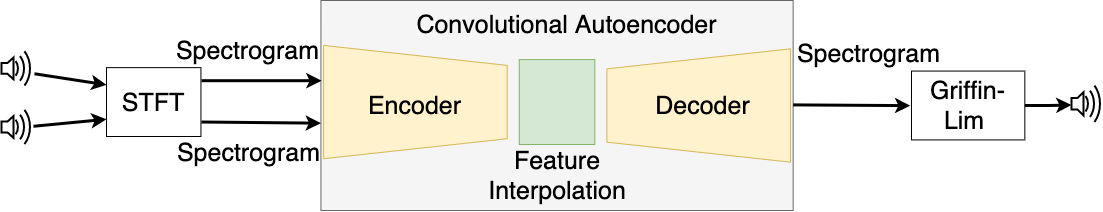
\includegraphics[width=\textwidth]{images/approach/Toolchain.png}
\end{figure}


\section{Pre Processing}

\section{ML-Model}

\section{Interpolation in latent space}

\section{Post Processing}

\section{Dataset}